\begin{document}
PM001-Atividade4
Diogo Takamori Barbosa
25/06

=
=============================================================================================
=
\textbf{1 - Dê exemplo de dois operadores ortogonais em R² cujas matrizes em relação à base canônica tenham na primeira coluna um vetor que é múltiplo dos dois maiores dígitos do seu RA. Explicite se estes operadores são uma rotação de um determinado ângulo (qual ?) ou são uma reflexão através de uma reta (qual?) Ilustre no computador o efeito destas transformações.}
-
Para encontrar dois operadores ortogonais em \(\mathbb{R}^2\) cujas matrizes em relação à base canônica tenham na primeira coluna um vetor que é múltiplo de \(\begin{pmatrix} 7 \\ 8 \end{pmatrix}\), e determinar se estes operadores são rotações ou reflexões.
As matrizes ortogonais \(A\) em \(\mathbb{R}^2\) têm a propriedade de que \(A^TA = I\), onde \(I\) é a matriz identidade. Também, para uma matriz ortogonal \(A\), as colunas de \(A\) são vetores ortonormais. 
Considerando que a primeira coluna é um múltiplo de \(\begin{pmatrix} 7 \\ 8 \end{pmatrix}\), podemos normalizar este vetor para obter um vetor unitário:
\[
   \vec{v} = \begin{pmatrix} 7 \\ 8 \end{pmatrix}
\]\[
   \|\vec{v}\| = \sqrt{7^2 + 8^2} = \sqrt{49 + 64} = \sqrt{113}
\]
o vetor unitário \(\vec{u}\) correspondente a \(\vec{v}\) é:
\[
   \vec{u} = \frac{1}{\sqrt{113}} \begin{pmatrix} 7 \\ 8 \end{pmatrix}
\]
Como a matriz é ortogonal, a segunda coluna precisa ser um vetor ortogonal a \(\vec{u}\) e também unitário. Seja \(\vec{w}\) o vetor ortogonal a \(\vec{u}\):
   \[
   \vec{w} = \frac{1}{\sqrt{113}} \begin{pmatrix} -8 \\ 7 \end{pmatrix}
   \]
Dessa forma, uma matriz ortogonal \(A\) pode ser formada por essas colunas:
\[
A_1 = \left(\begin{array}{cc} \frac{7}{\sqrt{113}} & \frac{-8}{\sqrt{113}} \\ \frac{8}{\sqrt{113}} & \frac{7}{\sqrt{113}} \end{array}\right)
\]
Esta matriz é uma matriz de rotação por um ângulo \(\theta\) tal que:
\[
\cos \theta = \frac{7}{\sqrt{113}}, \quad \sin \theta = \frac{8}{\sqrt{113}}
\]
Ângulo da rotação:
\[
\theta = \arccos\left(\frac{7}{\sqrt{113}}\right)
\]
Agora, para uma matriz de reflexão, a primeira coluna ainda deve ser um múltiplo de \(\begin{pmatrix} 7 \\ 8 \end{pmatrix}\), mas a segunda coluna será alterada para manter a ortogonalidade e a propriedade de reflexão:
\[
A_2 = \left(\begin{array}{cc} \frac{7}{\sqrt{113}} & \frac{8}{\sqrt{113}} \\ \frac{8}{\sqrt{113}} & -\frac{7}{\sqrt{113}} \end{array}\right)
\]
Esta matriz representa uma reflexão através da linha que faz um ângulo \(\theta\) com o eixo \(x\), onde:
\[
\theta = \arctan\left(\frac{8}{7}\right)
\]
Para ilustrar o efeito dessas transformações:
-
Matriz de rotação \(A_1\):
    - Esta matriz rotaciona vetores no plano por um ângulo \(\theta\).
    - Ilustração do efeito desta transformação:
 -
Matriz de reflexão \(A_2\):
    - Esta matriz reflete vetores através da linha que faz um ângulo \(\theta\) com o eixo \(x\).
    - Ilustração do efeito desta transformação:
 -
Código em Python para gerar as ilustrações:
 -
        \textit{import numpy as np
        import matplotlib.pyplot as plt
        -
        # Definir as matrizes
        theta_rotation = np.arccos(7/np.sqrt(113))
        A_1 = np.array([[7/np.sqrt(113), -8/np.sqrt(113)],
                        [8/np.sqrt(113),  7/np.sqrt(113)]])
        -
        theta_reflection = np.arctan(8/7)
        A_2 = np.array([[ 7/np.sqrt(113),  8/np.sqrt(113)],
                        [ 8/np.sqrt(113), -7/np.sqrt(113)]])
        -
        # Pontos originais
        points = np.array([[1, 0], [0, 1], [1, 1], [-1, -1], [-1, 1], [1, -1]])
        
        # Aplicar as transformações
        rotated_points = points @ A_1.T
        reflected_points = points @ A_2.T
        -
        # Plotar os pontos
        fig, ax = plt.subplots(1, 2, figsize=(14, 6))
        
        # Rotação
        ax[0].quiver(0, 0, points[:, 0], points[:, 1], angles='xy', scale_units='xy', scale=1, color='blue', alpha=0.5)
        ax[0].quiver(0, 0, rotated_points[:, 0], rotated_points[:, 1], angles='xy', scale_units='xy', scale=1, color='red', alpha=0.5)
        ax[0].set_xlim(-2, 2)
        ax[0].set_ylim(-2, 2)
        ax[0].axhline(0, color='black',linewidth=0.5)
        ax[0].axvline(0, color='black',linewidth=0.5)
        ax[0].grid(color = 'gray', linestyle = '--', linewidth = 0.5)
        ax[0].set_aspect('equal', adjustable='box')
        ax[0].set_title('Rotation by θ')
        
        # Reflexão
        ax[1].quiver(0, 0, points[:, 0], points[:, 1], angles='xy', scale_units='xy', scale=1, color='blue', alpha=0.5)
        ax[1].quiver(0, 0, reflected_points[:, 0], reflected_points[:, 1], angles='xy', scale_units='xy', scale=1, color='red', alpha=0.5)
        ax[1].set_xlim(-2, 2)
        ax[1].set_ylim(-2, 2)
        ax[1].axhline(0, color='black',linewidth=0.5)
        ax[1].axvline(0, color='black',linewidth=0.5)
        ax[1].grid(color = 'gray', linestyle = '--', linewidth = 0.5)
        ax[1].set_aspect('equal', adjustable='box')
        ax[1].set_title('Reflection through line at θ')
        
        plt.show()}
-
Ilustrações Geradas:
 -
Matriz de Rotação \(A_1\):
- Vetores originais em azul
- Vetores rotacionados em vermelho
\begin{figure}
    \centering
    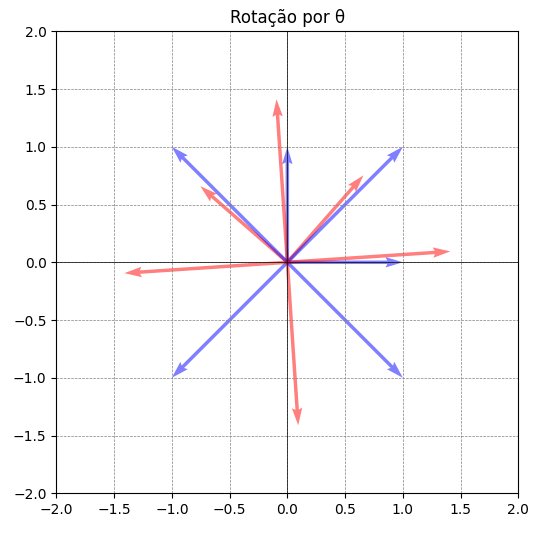
\includegraphics[width=0.75\linewidth]{image7.png}
\end{figure}
Matriz de Reflexão \(A_2\):
- Vetores originais em azul
- Vetores refletidos em vermelho
\begin{figure}
    \centering
    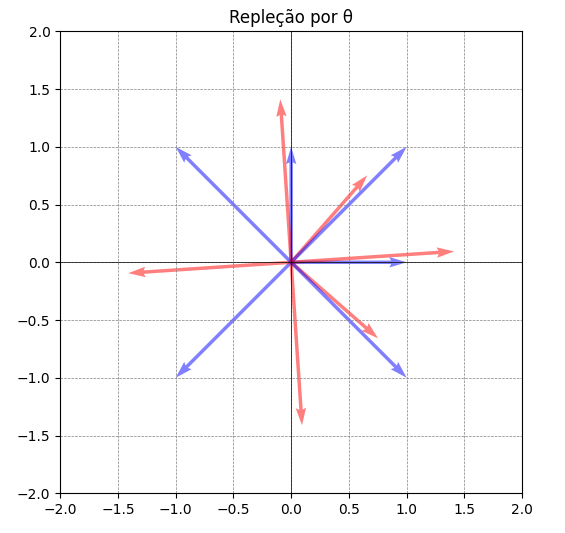
\includegraphics[width=0.75\linewidth]{image8.png}
\end{figure}
Etapas da 
Normalizar o vetor \(\begin{pmatrix} 7 \\ 8 \end{pmatrix}\)
\[
\|\vec{v}\| = \sqrt{113}
\]
\[
\vec{u} = \frac{1}{\sqrt{113}} \begin{pmatrix} 7 \\ 8 \end{pmatrix}
\]
Determinar vetor ortogonal unitário
\[
\vec{w} = \frac{1}{\sqrt{113}} \begin{pmatrix} -8 \\ 7 \end{pmatrix}
\]
Formar matriz de rotação e matriz de reflexão
\[
A_1 = \left(\begin{array}{cc} \frac{7}{\sqrt{113}} & \frac{-8}{\sqrt{113}} \\ \frac{8}{\sqrt{113}} & \frac{7}{\sqrt{113}} \end{array}\right)
\]
\[
A_2 = \left(\begin{array}{cc} \frac{7}{\sqrt{113}} & \frac{8}{\sqrt{113}} \\ \frac{8}{\sqrt{113}} & -\frac{7}{\sqrt{113}} \end{array}\right)
\]
- A matriz \(A_1\) é uma rotação por \(\theta = \arccos\left(\frac{7}{\sqrt{113}}\right)\)
- A matriz \(A_2\) é uma reflexão através da linha que faz um ângulo \(\theta = \arctan\left(\frac{8}{7}\right)\) com o eixo \(x\).
=
==========================================================================================
=

\end{document}

